% Created 2018-04-05 Thu 14:13
% Intended LaTeX compiler: pdflatex
\documentclass[11pt]{article}
\usepackage[utf8]{inputenc}
\usepackage[T1]{fontenc}
\usepackage{graphicx}
\usepackage{grffile}
\usepackage{longtable}
\usepackage{wrapfig}
\usepackage{rotating}
\usepackage[normalem]{ulem}
\usepackage{amsmath}
\usepackage{textcomp}
\usepackage{amssymb}
\usepackage{capt-of}
\usepackage{hyperref}
\hypersetup{colorlinks=true,urlcolor=blue,linkcolor=blue,pdfborder={0 0 0}}
\usepackage[english]{babel} % English language/hyphenation
\author{William Denton}
\date{\today}
\title{Easy Weeder}
\hypersetup{
 pdfauthor={William Denton},
 pdftitle={Easy Weeder},
 pdfkeywords={},
 pdfsubject={},
 pdfcreator={Emacs 27.0.50 (Org mode 9.1.6)},
 pdflang={English}}
\begin{document}

\maketitle

\section*{About}
\label{sec:org05083f2}

Easy Weeder is an algorithm that identifies little-used multiple copies of books and recommends how many copies we really need (minimum 1).

\section*{Busy factor}
\label{sec:orgb7b37c8}

The \emph{busy factor} will determine which books with multiple copies can be easily weeded.

First note that our calculations will be based on circs in a ``circ window'' of five years: the last five full academic years, plus the current year to date (so near the end of an academic year this will be almost six years).  In April 2018 the circ window includes all of academic 2012, 2013, 2014, 2015, 2106 and also academic 2017 from September 2017 to March 2018.

This means we know three things for each title:

\begin{itemize}
\item the number of copies (this is actually ``number of items with the same call number,'' so multiple copies of the same title are counted together, but four separate volumes in a four-volume set are not);
\item the number of circs of all those copies in the circ window; and
\item the length of circ window (defined as 5 years).
\end{itemize}

We can combine these into a measure of ``circs per copy per year,'' or how many times a year (on average, over the last five years) each copy of a title circulates.

Define the \emph{busy factor} to be number of circs divided by number of copies divided by length in years of the circ window.

\begin{equation}
\label{eq:org650bb63}
busy = \frac{\frac{circs}{copies}}{years}
\end{equation}

Some examples:

\begin{center}
\begin{tabular}{rrrr}
circs & copies & window & busy\\
\hline
10 & 1 & 5 & 2\\
5 & 1 & 5 & 1\\
7 & 2 & 5 & 0.7\\
2 & 1 & 5 & 0.4\\
1 & 2 & 5 & 0.4\\
2 & 19 & 5 & 0.02\\
698 & 2 & 5 & 69.8\\
\end{tabular}
\end{center}

The last two are real examples: Francis Bacon's \emph{\href{https://www.library.yorku.ca/find/Record/567179}{Advancement of Learning, and New Atlantis}} has a busy factor of 0.02, and \emph{\href{https://www.library.yorku.ca/find/Record/2914459}{Economics: Canada in the Global Environment}} is at 69.8, probably because it used to be on reserve but is now in the stacks.

Further, let us set a \emph{target busy factor} of 1.  That means in an ideal situation, if we have more than one copy of a book, each is used once a year.  (If we only have one copy of a title then Easy Weeder is not used, so its busy factor is not used.)

\section*{Assumptions}
\label{sec:orgddafa39}

\begin{enumerate}
\item We don't keep two copies of a book in the circulating collection just in case one gets lost.
\item To minimize human oversight, we will always keep at least 1 copy of a title.  Weeding all copies of a title goes beyond Easy Weeder's scope.
\item The inventory is accurate.  (If it is not, it can be corrected as weeding is done, and anyway that would rarely affect the number of copies that Easy Weeder will recommend: if we think we have four copies of something but only need one, it doesn't matter that really we only have three.)
\end{enumerate}

\section*{How the logic and calculations work}
\label{sec:org072678e}

\begin{figure}[htbp]
\centering
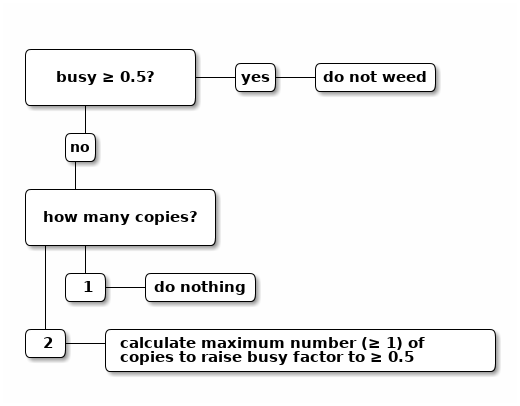
\includegraphics[height=3in]{logic-flow.png}
\caption{\label{fig:org9385754}
Easy Weeder logic}
\end{figure}

To revisit the examples above, two are ignored because their busy factor is >= 1.  For the remaining four we can calculate the recommended number of copies we should keep.  Figure \ref{fig:org9385754} shows the decisions made.

For example, for the one with 19 copies, and 2 circs, the calculation goes:

\begin{itemize}
\item 19 copies is too many.  18 → busy = 0.022.
\item 18 copies is too many.  17 → busy = 0.024.
\item …
\item 5 copies is too many.  4 → busy = 0.1.
\item 4 copies is too many.  3 → busy = 0.133.
\item 3 copies is too many.  2 → busy = 0.2.
\item 2 copies is too many. Keep 1 copy.
\end{itemize}

As it happens, for all four we end up keeping just one copy.

\begin{center}
\begin{tabular}{rrrrr}
circs & copies & window & busy & rec\_copies\\
\hline
7 & 2 & 5 & 0.7 & 1\\
2 & 1 & 5 & 0.4 & 1\\
1 & 2 & 5 & 0.4 & 1\\
2 & 19 & 5 & 0.02 & 1\\
\end{tabular}
\end{center}

But, for example, let's say we had a book that had 6 copies and 12 circs over the last 5 years, for a busy factor of 0.4.  We would keep 2 copies.

\begin{itemize}
\item 6 copies is too many.  5 → busy = 0.48.
\item 5 copies is too many.  4 → busy = 0.6.
\item 4 copies is too many.  3 → busy = 0.8.
\item 3 copies is too many.  2 → busy = 1.2.
\item Keep 2 copies.  (2 is the largest number giving a busy factor >= 1.)
\end{itemize}

\section*{Estimated easy weedables (April 2018)}
\label{sec:orgbb92aee}

\subsection*{Space measurements}
\label{sec:org1fb5084}

Rules of thumb for how many books fit into a space:

\begin{center}
\begin{tabular}{lll}
30 books & is & 1  shelf\\
7 shelves & is & 1 stack\\
10 stacks & is & 1 range\\
2 ranges & is & 1 row\\
\end{tabular}
\end{center}

Therefore, one stack holds \(30 \times 7 = 210\) books, one range holds \(210 \times 10 = 2100\) books and one row holds \(2100 \times 2 = 4200\) books.  Some ranges have fewer stacks, and some shelves hold more books, but these are good enough for estimates.

\subsection*{By branch}
\label{sec:org71cf9ee}

\begin{center}
\begin{tabular}{lrrr}
home\_location & n & stacks & rows\\
\hline
BRONFMAN & 842 & 4 & 0\\
FROST & 2050 & 10 & 0\\
LAW & 602 & 3 & 0\\
SCOTT & 117069 & 557 & 28\\
STEACIE & 883 & 4 & 0\\
\end{tabular}
\end{center}

\subsection*{By branch and class letter}
\label{sec:orgaf3c064}

\begin{longtable}{lrrrrr}
lc\_letter & BRONFMAN & FROST & LAW & SCOTT & STEACIE\\
\hline
\endfirsthead
\multicolumn{6}{l}{Continued from previous page} \\
\hline

lc\_letter & BRONFMAN & FROST & LAW & SCOTT & STEACIE \\

\hline
\endhead
\hline\multicolumn{6}{r}{Continued on next page} \\
\endfoot
\endlastfoot
\hline
A &  &  &  & 308 & \\
B &  & 89 & 2 & 14612 & \\
C &  & 2 &  & 1095 & 2\\
D &  & 83 & 1 & 9966 & 1\\
E &  & 43 & 5 & 4382 & \\
F &  & 383 & 5 & 8300 & \\
G & 1 & 12 &  & 5296 & 16\\
H & 816 & 433 & 80 & 20388 & 32\\
J & 1 & 156 & 17 & 2645 & \\
K & 2 & 13 & 411 & 1372 & 3\\
L & 1 & 10 & 5 & 2325 & 1\\
M &  & 1 &  & 1461 & 1\\
N & 3 & 13 & 2 & 6751 & \\
P & 2 & 757 & 7 & 30113 & 1\\
Q & 1 & 21 &  & 743 & 568\\
R & 2 & 16 & 8 & 5012 & 150\\
S &  & 2 &  & 157 & 19\\
T & 13 & 5 & 2 & 769 & 79\\
U &  & 9 &  & 737 & 1\\
V &  &  &  & 44 & \\
X &  &  & 46 &  & \\
Z &  & 2 & 11 & 593 & 9\\
\end{longtable}

\section*{To note}
\label{sec:org23f6e72}

\begin{itemize}
\item Easy Weeder does not use acquisition year.  Low-circing multiple copies acquired within the last 5 years may need a human decision.
\item Easy Weeder does not remove duplicates across branches, but the same data can be used to do that. For example, \emph{\href{https://www.library.yorku.ca/find/Record/1172}{Captains of Consciousness: Advertising and the Social Roots of the Consumer Culture}} has ten copies at three branches: Bronfman (7), Frost (1) and Scott (2).  Circulation in the circ window is: Bronfman (13), Frost (0), Scott (15).  Therefore Easy Weeder recommends this number of copies: Bronfman (2), Frost (1) and Scott (2).  Even if it makes sense to have the book at both Bronfman and Scott (which would need 3 copies to get down to a busy factor of 1), Frost does not need a copy, because no one has used it there since 2010.
\end{itemize}

\section*{Commands}
\label{sec:org82aed90}

\begin{description}
\item[{\texttt{make}}] prepare the Easy Weeder data
\item[{\texttt{make get\_data}}] use locally to pull down production Easy Weeder data
\item[{\texttt{make push\_app}}] use locally to push the Shiny app up to production
\end{description}

\section*{Installation}
\label{sec:org6be31a8}
\end{document}
